
\documentclass[12pt]{report}         
\usepackage {utthesis2}              
\usepackage[utf8]{inputenc}
\usepackage{tocloft}
%\usepackage{ulem}
%\usepackage{setspace}
\usepackage[left=1in, right=1in]{geometry}
\usepackage{graphicx}
\usepackage[document]{ragged2e}
\usepackage{tabularx}
\usepackage{amsmath}
\usepackage{algorithmic}
%\usepackage[ruled]{algorithm2e}
\usepackage{ragged2e}
\usepackage{fancyhdr}
\usepackage{listings}
\pagestyle{plain}
\usepackage{algorithm}
\usepackage{hyperref}
\hypersetup{
    colorlinks=true,
    linkcolor=black,
    filecolor=black,      
    urlcolor=black,
}

\usepackage{xcolor}

\definecolor{codegreen}{rgb}{0,0.6,0}
\definecolor{codegray}{rgb}{0.5,0.5,0.5}
\definecolor{codepurple}{rgb}{0.58,0,0.82}
\definecolor{backcolour}{rgb}{0.95,0.95,0.92}

\lstdefinestyle{mystyle}{
    backgroundcolor=\color{backcolour},   
    commentstyle=\color{codegreen},
    keywordstyle=\color{magenta},
    numberstyle=\tiny\color{codegray},
    stringstyle=\color{codepurple},
    basicstyle=\ttfamily\footnotesize,
    breakatwhitespace=false,         
    breaklines=true,                 
    captionpos=b,                    
    keepspaces=true,                 
    numbers=left,                    
    numbersep=5pt,                  
    showspaces=false,                
    showstringspaces=false,
    showtabs=false,                  
    tabsize=2
}

\lstset{style=mystyle}

\mastersthesis                     
\onehalfspacing                   

\renewcommand{\thesisauthor}{Animesh Goyal}    

\renewcommand{\thesismonth}{May}     

\renewcommand{\thesisyear}{2020}     

\renewcommand{\thesistitle}{Multi-Agent Deep Reinforcement Learning for RoboCup Rescue Simulator}   

\renewcommand{\thesissupervisor}{Peter Stone}
                                     
\renewcommand{\thesiscosupervisor}{Garrett Warnell}
                                    

\renewcommand{\thesisauthoraddress}{4305 Duval St. 78751, Austin, TX, USA}
                                     

\renewcommand{\thesisdegree}{Master of Science in Operation Research and Industrial Engineering } 

\renewcommand{\thesistype}{Master's Report}    

%%%
%%%%%%%%%%%%%%%%%%%%%%%%%%%%%%%%%%%%%%%%%%%%%%%%%%%%%%%%%%%%%%%%%%%%%%%%%%%%%

\begin{document}
\justify 
\noindent

\thesiscopyrightpage                 

\thesiscertificationpage             

\thesistitlepage                     

%\thesissignaturepage               

% \thesisdedicationpage               

\begin{thesisacknowledgments}       
First and foremost I would like to thank my advisor, Peter Stone, for his guidance and encouragement throughout this report. He always made himself available to provide help and I could always count on his lightning-fast email responses. He gave me autonomy in finding a research topic and provided the right amount of guidance to help me make progress when I felt stuck. It has been a privilege to work with him. Garrett Warnell and Tsz-Chiu Au deserves a special thanks as collaborators and mentors throughout my research. They have provided invaluable help, especially with regards to their extensive reviews of my writing. Discussions with them have helped me flesh out ideas fully, and my writing and research ability have improved through their mentorship.    

I would like to thank several of my peers and colleagues for the help they’ve provided during my report. Aastha Goyal has provided invaluable input with her experience in Java and gRPC. She was always been very helpful and supportive. Ashutosh Shukla reviewed several of my work and provided extensive feedback. His constant motivation was very encouraging throughout my research. I would also like to thank Ishan Durugkar and Siddharth for being always available to solve any doubts that I had regarding the simulator. 

This work has taken place in the Learning Agents Research Group (LARG) at the Artificial Intelligence Laboratory, The University of Texas at Austin.  LARG research is supported in part by grants from
the National Science Foundation (CPS-1739964, IIS-1724157, NRI-1925082), the Office of Naval Research (N00014-18-2243), Future of Life Institute (RFP2-000), Army Research Laboratory, DARPA, Lockheed
Martin, General Motors, and Bosch.  Peter Stone serves as the Executive Director of Sony AI America and receives financial compensation for this work.  The terms of this arrangement have been reviewed and approved by the University of Texas at Austin in accordance with its policy on objectivity in research. 

\end{thesisacknowledgments}          

\begin{thesisabstract}               

Recent advancement in the field of Artificial Intelligence have dealt with creating a winning strategy for games like Atari, DOTA 2 and StarCraft where agents learn how to finish their task successfully using reinforcement learning. As the capabilities have increased, the research community has sought games having increased complexity that seize different aspects of intelligence required to solve real-world problems. 

Large state space analysis and long term planning are one of the core requirements of strategic games in order to build a winning strategy. Building these winning strategies using deep reinforcement learning is a attractive as well as challenging task to work on specially when it incorporates multi-agent training where building the strategy is even more difficult. Applying deep reinforcement learning to such multiagent scenario is together known as Multiagent Deep Reinforcement learning (MADRL). 

In this work, we apply MADRL to RoboCup Rescue Simulator (RCRS), which is part of the annual RoboCup Competition. RCRS is an open-source virtual environment that evaluates how effective multiple agents like ambulance team, police officer and fire brigades are in rescuing civilians and extinguishing fire from a city where an earthquake just happened. RCRS is challenging, easy to use and customize multi-agent scenario. 

In order to create RCRS environment where reinforcement learning algorithms can be tested, RCRS-gym, an open-source OpenAI Gym environment was created. We tested various algorithms for different map settings where number of agents and buildings were changed. 

Using two DRL algorithms, Deep Q-Network and Proximal Policy Optimization, we were able to train the agents to successfully finish the task of extinguishing fire on the "Small" map thus proving that RCRS is a suitable environment for developing deep reinforcement learning agent in a strategic multiagent game scenario. "Big" map required more training time to make conclusions on the agent's final performance. 
                                
\end{thesisabstract}                 

\tableofcontents                     

\newpage

\addcontentsline{toc}{chapter}{List of Figures}%
\listoffigures
\newpage
\addcontentsline{toc}{chapter}{List of Algorithms}%
\listofalgorithms
\newpage
\addcontentsline{toc}{chapter}{List of Tables}%
\listoftables
\newpage

\chapter{Introduction}            

On April 2019, OpenAI's DOTA 2 beat 99.4 percent of players in public matches \cite{dota2}. On October 2019, DeepMind's StarCraft II AI was able to play better than 99.8 percent of all humans \cite{Starcraft2}. These are milestone achievements where artificial intelligence has been used in the area of Multi Agent Systems (MAS). Although different techniques and algorithms were used in the above scenarios, in general, they are all a combination of techniques from two main areas: Reinforcement Learning and Deep Learning. 

Reinforcement learning (RL) is an area of machine learning where agents learn what actions to take in certain environment that results in higher cumulative reward over time. However, one of the drawbacks of RL is that the state space or action space can become too large to be completely known. This is where neural networks can be particularly useful as they are very good function approximators. Neural Networks can learn to map states values, or state-action pairs to Q values. Rather than building a lookup table to store, index and update all possible states and their values, we can train a neural network on samples from the state or action space to learn to predict how valuable those are relative to our target in reinforcement learning. This is called Deep Reinforcement learning (DRL). 

\begin{figure}[!h]
    \centering
    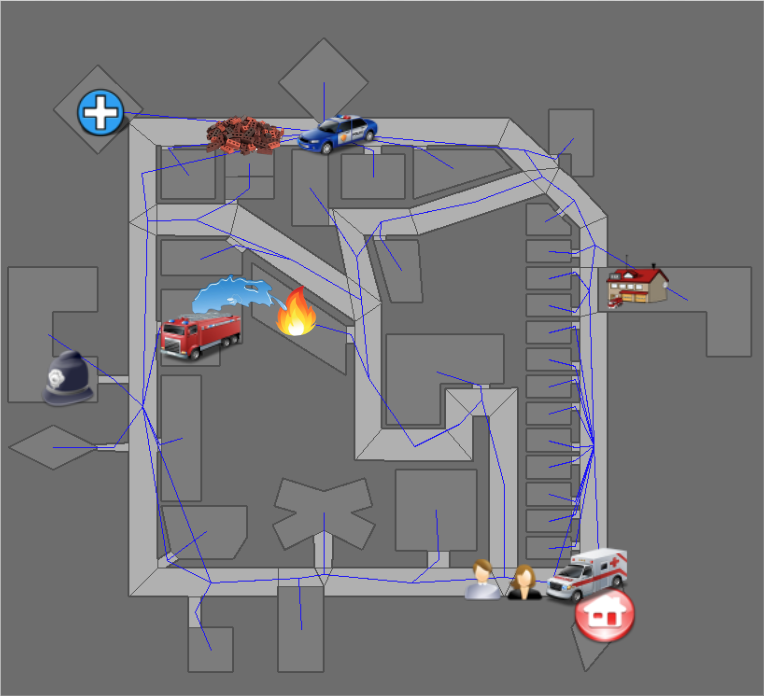
\includegraphics[width=12cm]{10.png}
    \caption{\textbf{RoboCup Rescue Simulation Environment:} RoboCup Rescue Simulator provides a 2D reinforcement learning environment where agents can be trained to save civilians and extinguish fire in a city where an earthquake has taken place}
    \label{fig:10}
\end{figure}

Together MAS and DRL are referred to as Multiagent Deep Reinforcement learning (MADRL). Currently, most of the work done in MADRL has been done in the field of video games (e.g. Atari games) and there is still a lot of work to be done for more realistic applications with complex dynamics, which are not necessarily vision based. 

One such domain is RoboCup Rescue Simulator (RCRS) (Figure ~\ref{fig:10}). RCRS is structured as a 2D discrete-time simulation system that depicts the situation after occurrence of earthquake in an urban area. Different agents like police officers, fire brigades and ambulance teams interact with the environment and with each other to accomplish tasks such as removing blockades, extinguishing fire and rescuing civilians. This task allocation can be handles in two ways: centralized or distributed. In centralized task allocation, a central agent manages all the agents and has the global knowledge whereas in case of distributed task allocation problem, each agent makes its own decisions and works only on its local information \cite{Nair}. 

\textbf{Contributions:} In this report, using centralized task allocation approach we have applied Deep Reinforcement Learning (DRL) algorithms to RCRS in order to train multiple fire brigades to extinguish the fire in the city on different sized maps having different number of agents and total buildings. The major contributions are listed below: 

\begin{itemize}
    \item Built a RCRS-Gym interface, that can be utilized to apply various reinforcement learning algorithms to RCRS
    \item Evaluated state-of-the-art reinforcement learning algorithms on RCRS, providing an extensive set of results for comparison
    \item Successfully trained the agents to learn a winning strategy thus proving that RCRS is a suitable environment for applying DRL 
    \item Showcased promising future research directions in this environment i.e. partial observability and including police officer and ambulance as the agent
\end{itemize}

The rest of the report is structured as follows. Chapter 2 will help build important concepts that are important for understanding this project. Specifically it will explain the state-of-art DRL algorithms. In Chapter 3, detailed explanation of the simulator is done along with the state space, action space and reward function selected. In Chapter 4, implementation of the model in RCRS will be detailed along with the results. In Chapter 5, everything will be summarized and will discuss the future directions for the project. 


\chapter{Background}                       

This chapter will briefly cover the basic but very important concepts like Reinforcement learning, Deep Reinforcement learning and Multi-agent system that will build the necessary background to understand the project properly.  

\section{Reinforcement learning}

Reinforcement learning is modeled as a Markov decision process where the agent interacts with the environment to learn the actions in a certain state which would produce the highest reward. The reinforcement learning model is depicted in Figure ~\ref{fig:ReinforcementLearningModel} 

\begin{figure}[!h]
    \centering
    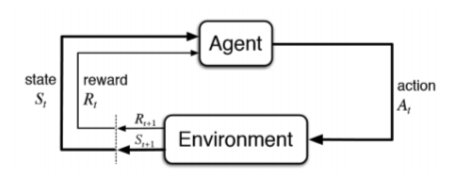
\includegraphics[width=12cm]{ReinforcementLearningModel.png}
    \caption{Abstract depiction of reinforcement Learning Model: At some point in time t, the RL agent experiences a state $S_t$ and a reward $R_t$ for his action in time $t-1$. In state $S_t$, the agent takes action $A_t$ , for which the environment advances a time step, and the agent experiences a new state $S_{t+1}$ and a reward $R_{t+1}$ for action $A_{t+1}$}
    \label{fig:ReinforcementLearningModel}
\end{figure}

In order to maximize the long term reward signal, Reinforcement learning learns optimal actions for specific environment conditions by trial-and-error \cite{Barto}. 

At each time step t, the agent perceives a state $S_t$ in state space S from which it selects an action $A_t$ in the action space A by following a policy $\pi$. The agent receives a reward $R_t$ when it transitions to the state $S_{t+1}$ according to the environment dynamics, the reward function R($S_t$, $A_t$, $S_{t+1}$) and the transition function T($S_t$, $A_t$, $S_{t+1}$). Discount factor $\gamma$ $\in$ [0, 1] is applied to the future rewards. There are two types of RL approach: model based and model free. 

\textbf{Model based approach} uses a reduced number of interactions with the real environment during the learning phase. Its aim is to construct a model based on these interactions, and then use this model to simulate the further episodes, not in the real environment but by applying them to the constructed model and get the results returned by that model.

\textbf{Model free based approach} act in real environment in order to learn. The most common model-free technique is Q-Learning and Policy Gradient methods. For our project, we will focus on Model free based approach since agents will have to learn by acting in the real RCRS environment. 

\subsection{Q-learning} In Q-learning we are trying to build a Q-table that stores all possible combinations of state S and action A. Q value will be depicted as Q(S,A). We sample an action A from the Q-table for the current state S and observe the reward R and next state S'. Then from the Q-table we determine the next action A' in order to have maximum Q(S', A') (Figure ~\ref{fig:QLearning}). 

\begin{figure}[!h]
    \centering
    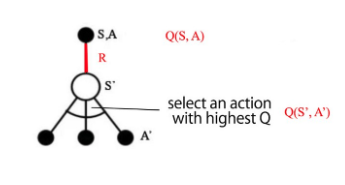
\includegraphics[width=8cm]{QLearning.png}
    \caption{Working of Q-Learning}
    \label{fig:QLearning}
\end{figure}

\[ Target = R(S,A,S') + \gamma \max_{\{A'\}} Q_k (S', A')  \] 

Here $\gamma$ is the discount factor with values lying between [0,1]. It controls the importance of future rewards vs the immediate ones. The lower the discount factor, the lesser important future rewards are and the agent will tend to focus on actions that will yield immediate rewards.    

\subsection{Policy Gradient} Policy gradient doesn't calculate the Q-value but instead uses a policy. 

\[ \pi_\theta (a | s) = P [ a | s ] \]

The policy learns a mapping from every state to action, and its objective is to find which actions lead to higher rewards and increase their probability. 

Policy gradient observes the environment and acts in it and keeps updating its policy based on the rewards it receives. 

\[ \tau = (s_1, u_1, s_2, u_2, ....., s_h, u_h ) \]

The objective function for policy gradient is:
\[ J(\theta) = E[\sum_{t=0}^{H} R(s_t, u_t); \pi_\theta] = \sum_{\tau} P(\tau;\theta) R(\tau) \] 

After multiple iterations, policy converges to a maximum value. Drawbacks of policy gradient method can be that it sometimes can get stuck in local maximum and will not be able to reach the global maximum.  

\section{Deep Reinforcement learning}

In situations where there is large state and action space, it is not feasible to learn the Q-values or a policy for each state and action pair. This is when Deep Reinforcement learning (DRL) is used where neural networks are utilized to model the components of RL. A representation of the architecture is given in Figure ~\ref{fig:DRLArchitecture}. 

\begin{figure}[!h]
    \centering
    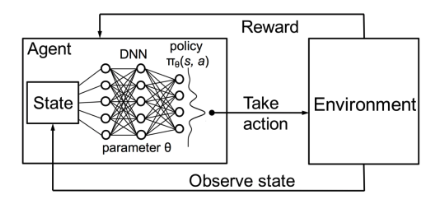
\includegraphics[width=12cm]{DRLArchitecture.png}
    \caption{Deep Reinforcement learning Architecture \cite{Mao}}
    \label{fig:DRLArchitecture}
\end{figure}


We consider two DRL model free based algorithms: Deep Q-Learning and Proximal Policy Optimization mainly because DQN showed great results on Atari games and helped the team achieve human level performance whereas using PPO, OpenAI's DOTA 2 team was able to beat 99.4 percent of players in a public match.  \\

\subsection{Deep Q-Networks(DQN)} DQN is a combination of Q-Learning and deep neural networks. DQN addresses the instabilities caused by using non-linear approximator to represent the Q-value by using two insights: experience replay and target network. 
Using Convolutional Neural Network (CNN) , DQN parameterizes an approximate value function Q(s, a; $\theta_i$) where $\theta_i$ are the weights of the network at iteration i. The experience replay stores the agent’s experiences $e_t$ = ($s_t$, $a_t$, $r_t$, $s_{t+1}$) at each time step t in a dataset $D_t$ = $e_1$,$e_t$ pooled over many episodes into a replay
memory. Then, mini batches of experience drawn uniformly at random from the dataset (s, a, r, s) $\sim$ U(D) are applied as Q-updates during the training. The
Q-learning update at iteration i follows the loss function:

\[ L_i (\theta_i) = E_{(s,a,r,s) \sim U(D) } [(r +  \gamma max_{a^{'}} Q(s^{'}, a^{'} ; \theta_i^{-}) - Q(s,a; \theta_{i}))^2] \]

\hfill \break
where $\theta_i$ are the Q-network parameters at iteration i and $\theta_i^{-}$  are the target network parameters. The target network parameters are updated with the Q network parameters every C steps and are held fixed between individual updates. \\

\subsection{Proximal Policy Optimization (PPO)} PPO is a type of policy gradient method which performs  comparably or better than state-of-the-art approaches while being much simpler to implement and tune. Careful tuning of the step size is required for achieving good results with policy gradient algorithms \cite{PPO}. Moreover, most policy gradient methods perform one gradient update per sampled trajectory and have high sample complexity. Schulman et al. \cite{Schulman} introduced PPO algorithm that solves both these problems. It uses a surrogate objective which is maximized while penalizing large changes to the policy. 
They defined a likelihood ratio 

\[ l_t(\theta) = \frac{\pi_\theta(a_t | s_t)}{\pi_{\theta old}(a_t | s_t)}\]

\hfill \break
PPO then optimizes the objective: 

\[ L^{CLIP} = \hat{E}_t [min(l_t(\theta) \hat{A}_t, clip(l_t (\theta) , 1- \epsilon , 1+\epsilon)\hat{A}_t)] \]

\hfill \break
where $\hat{A}_t$ is the generalized advantage estimate and $clip(l_t (\theta) , 1- \epsilon , 1+\epsilon)$ clips $l_t(\theta)$ in the interval [1 - $\epsilon$, 1 + $\epsilon$]. The algorithm alternates between sampling multiple trajectories from the policy and performing several epochs of SGD on the
sampled dataset to optimize this surrogate objective. Since the state value function is also simultaneously approximated, the error for the value function approximation is also added to the surrogate
objective to compute the complete objective function. 

\section{Multi-Agent Systems (MAS)}

In multi-agents systems there are several agents that model each other's goals and actions \cite{Stone}. There may be direct communication between the agents in a fully general multiagent scenario. In multiagent systems, environment dynamics of other agents can be known by each agent which is unlike single agent systems, other agents can affect the environment in unpredictable ways and can create uncertainty in the domain. Therefore, multiagent systems can be viewed as having dynamic environments. Figure ~\ref{fig:MultiAgentSystem} shows a fully general multiagent scenario. 

\begin{figure}[!h]
    \centering
    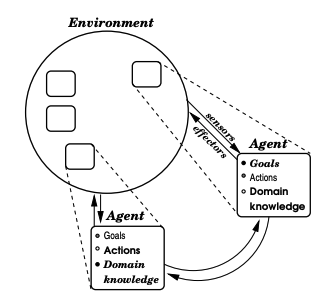
\includegraphics[width=12cm]{MultiAgentSystem.png}
    \caption{A fully general multiagent scenario. Agents can affect other agents actions, goals or domain knowledge or communicate directly with each other \cite{Stone}}
    \label{fig:MultiAgentSystem}
\end{figure}


Multiagent Systems can be further divided into various categories mentioned below \cite{SurveyandArticle}:

\begin{itemize}
    \item \emph{Goals}: Environment setting can be cooperative, competitive or mixed. In cooperative setting, all agents usually share a common reward function. Competitive setting is usually modelled as a zero-sum Markov game, where reward of one agent is exactly the loss of the other. Mixed setting is also known as the general-sum game setting where no restriction is imposed on the goal and relationship of the agents. Each agent is self interested and can have conflicting rewards.
    \item \emph{Actions}: Actions can be deterministic or stochastic. In case of deterministic actions, taking an action always results in the same action being taken whereas in case of stochastic actions, actions can change with a certain probability
    \item \emph{Domain knowledge}: The environment can be partially or fully observable. In partial observability, each agent has access to only certain information about the environment. 
\end{itemize}

For our case, environment is fully observable where all agents have total information about other agents and the environment as well. Its a cooperative setting where all agent have a common reward function. All the actions are deterministic in nature. 

\chapter{Related Work}

With the definitions set, we will now elaborate on the work that is so far done in the field of MADRL and how RL has been applied to RCRS.

\section{Multi-Agent Deep Reinforcement learning (MADRL)}

Since the success of deep RL using DQN proposed by \cite{Kavukcuoglu} many algorithms have been proposed to integrate deep learning to multiagent systems to solve complex problem in a variety of areas. This section provides a survey of these applications with a focus on the integration of deep learning and MARL. 

One of the earliest MADRL work was done by Tampuu et al \cite{Tampuu}. They had two independent DQN learning agents to play the Atari Pong game. They focused on building a reward function which resulted in either cooperative or competitive behaviours. Leibo et al. \cite{Leibo} studied about independent DQNs in the context of sequential social dilemmas which is a Markov game that satisfies certain inequalities. Their work focused on highlighting that cooperative or competitive behaviors exist not only as discrete actions but they are temporally extended over policies. Being able to capture sequential structure of real world social dilemmas, sequential social dilemma is an extension of matrix game social dilemma which has been previously applied to various phenomena in biology \cite{Cote}. DQN was used to find self interested independent learning agents to find equilibria of the sequential social dilemma which cannot be solved by the standard evolution methods used for matrix game social dilemma \cite{Weiner}. Lerer and Peysakhovich \cite{Lerer} were able to show theoretically and experimentally that agents can maintain cooperation using the famous Tit-for-Tat strategy for DRL (using function approximators). They used self play and two reward schemes: selfish and cooperative to construct the agents. Bansal et al. \cite{Bansal} used MuJoCo simulator to explore the emergent behaviors in competitive scenarios. They trained independent learning agents with PPO and incorporated two main modifications to deal with the Multiagent nature of the problem. Raghu et al. \cite{Raghu} studied how DRL algorithms like DQN, PPO performed in a two-player zero-sum games with tunable complexity called Erdos-Selfridge Spencer games. They were able to show that algorihms can exhibit wide variation in performance as the algorithms are tuned to the game's difficulty. Jiang and Lu \cite{Jiang} proposed a novel MADRL model that learns to communicate and exchange information while making decisions using actor-critic algorithm. Another interesting work in the field of MADRL was by Shao et al. \cite{Shao} for the game of StarCraft. In order to balance the units moved and attack strength of the enemy, they used parameter sharing multi-agent gradient descent SARSA algorithm using neural network to approximate the value function and reward function. However, high computation power was required for the implementation. 

\section{Reinforcement learning for RCRS}

On January 17th 1995, the Great Hanshin earthquake hit the Japanese port city Kobe with a magnitude of 6.8 on richter scale causing mass destruction taking approximately 7000 lives \cite{Bilski} \cite{RoboCup}. In response to the disaster, it was decided that the current disaster management policies should be changed. On April 30th 1999, RoboCup Rescue league was founded in order to promote international research towards the development of better rescue capabilities \cite{Bilski}.   

Over the years many teams have participated in the annual RoboCup Rescue league which consists of three competitions: robotics competition, virtual robot competition and the simulated agent competition. We will be focusing on the simulated agent competition known as RoboCup Rescue Simulation (RCRS) which is a perfect example of multiagent systems. 

In this section we will go over the work done by previous participating teams and how they have applied Reinforcement learning to RCRS. 

Martinez et. al \cite{Martinez} were the first one to implement Reinforcement Learning to RCRS. They introduced evolutionary reinforcement learning to improve the ambulance decision making process such as deciding the number of ambulances required to rescue a buried civilian. Their trained agent was able to outperform the participants of 2004 RCRS competition and was also computationally efficient. Visser et. al \cite{Visser2018RoboCupRS} developed a new framework to incorporate state-of-the-art machine learning algorithms into RoboCup Rescue competition code using the MATLAB Engine API for Java. They showed how supervised machine learning methods like classification and regression can be applied to assess the strategies of the agents and found the most relevant predictors. For example, estimating the chance of survival for a trapped civilian by predicting the remaining health point at the end of the scenario. Abdolmaleki et. al \cite{abdolmaleki} used SARSA to train the agent. They also proposed lesson-by-lesson learning which solved the problem of huge search space. Their proposed model increased the speed of learning and utilized very low memory. They discussed how temporal difference (TD) learning can be used to find the optimum policy for fire extinguishing tasks of a group of firefighter agents. Bitaghsir et. al \cite{Bitaghsir} introduced a layered neuro-fuzzy paradigm which is inspired from incremental learning. The paradigm was used for developing intelligent firefighter robots which involved layering increasingly complex learned behaviors. Aghazadeh et. al \cite{Aghazadeh} used parametric reinforcement learning to improve police force's decision making in RCRS. Using linear function approximator, they were able to perform the tasks using very less space. The work done till now has been quite intriguing but none of it involved MADRL to train the agents. This is what inspired us to write this report. 

\chapter{Modeling DRL for RCRS}

\section{Domain Description}

The competition is based on a complex simulation platform representing a city after an earthquake. In order to make the simulator as realistic as possible, its designed to have heterogeneous agents (different types of agent), limited reach (agents can only perform tasks occurring close to them), random fire spread, injured victims, agents having limited communication with messages often getting dropped, agents being only able to see a short distance. It is therefore considered as a multiagent simulator \cite{Kitano}.  

RCRS has 3 major parts: Environment, Agents and Line of Sight:

\subsection{Environment}

The RCRS environment comprises of various kinds of entities. The most important are buildings, roads, blockages, refuges and humans \cite{Morimoto}. 


\textbf{Buildings} are real constructions and have properties like area, fieryness and temperature, if its made of wood or cement. This information is useful for the simulator to calculate fire spread and building collapses. In case the building area is high and made of wood, fire will spread quickly. Simulator also changes the color of the building depending on the temperature and fieryness value. In case both the properties are high, color gets darker and eventually turning black if the building is burned out. Note that fieryness value means how strong the fire is. 

\textbf{Roads} help the agents to move along the map. Some of the properties of roads are length, number of lanes. If a road is blocked due to agents standing in front or blockages, its not possible to move along it. 

\textbf{Blockages} is the property of blocking the lanes which usually occurs because of debris falling on the roads after earthquake. This prohibits agents to move forward. The only agent that can clear these blockages is police officers. They have a property of repair cost which lets the police officer know how difficult it is to clear them. 

\textbf{Refuge} are buildings where Fire Brigades can refill their water tanks and civilians can be kept safely. These buildings do not catch fire or collapse. 

\subsection{Agents} There are 3 kinds of agents in RCRS. 

\textbf{Fire Brigades} These agents are responsible for extinguishing fires in the buildings. They have water tanks with certain water capacity that needs to refilled from the refuge. Fire Brigades also have health points that decreases in case they catch fire or enter a building on fire. In case there health points drops to zero, they are considered dead. 

\textbf{Ambulance Teams} These agents are responsible for rescuing the injured civilians and carrying them safely to the refuge. They also have health points that decreases in case they catch fire. They cannot carry more than one victim at a time. 

\textbf{Police Officers} These agents are responsible to clear the blockages and allow other agents to complete their tasks. To clear a blockage, police officers need to get close to it. 

Pictorial view of all the entities in the simulator are mentioned in Figure ~\ref{fig:RCRSActors}. 

\begin{figure}[!h]
    \centering
    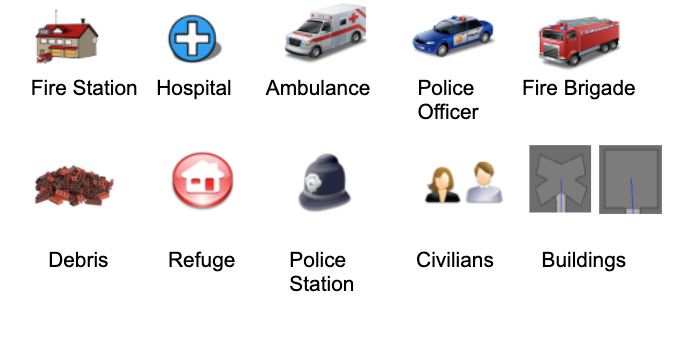
\includegraphics[width=12cm]{RCRSActors.png}
    \caption{Entities in RoboCup Rescue Simulator}
    \label{fig:RCRSActors}
\end{figure}

\hfill

In this report, we have focused on training multiple fire brigades to extinguish the fire as quickly as possible. Figure ~\ref{fig:RepresentationofSimulator} gives a visual representation of how the simulator looks. 

\begin{figure}[!h]
    \centering
    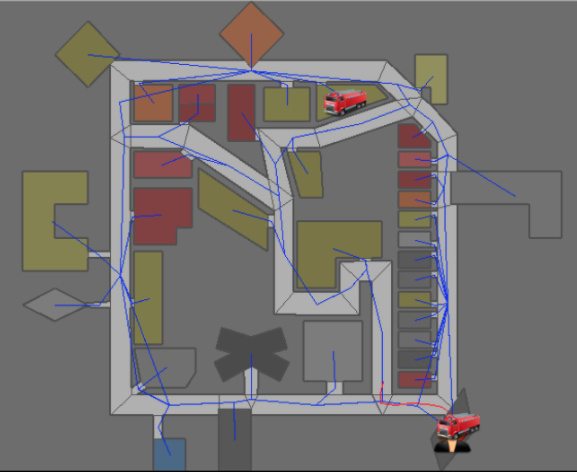
\includegraphics[width=12cm]{13}
    \caption{\textbf{Representation of the Simulator:} RoboCup Rescue Simulator with fire brigades. Different polygons are the buildings in the map. Grey color shows building is unburnt, yellow and red color shows building is burning, blue color depicts fire is extinguished and black shows the building is totally burnt. Note that as the shades get darker, building temperature and fieryness (degree of fire) increases.}
    \label{fig:RepresentationofSimulator}
\end{figure}

\subsection{Search Strategy of Fire Brigades}

Fire is initiated randomly following a Poisson distribution. Fire brigades start searching the map looking for fire spots in the environment. Once the fire trucks detect a fire, they start extinguishing it. Note that extinguishing only takes place if the fire trucks are in a close proximity to the building. Fire brigades extinguish the fire until one of the three conditions hold true: (i) It is able to extinguish the fire completely, (ii) building has been completely burned out, or (iii) water in the fire tank is empty. For the first two situations, fire brigades start searching for a new building. For the third case, fire brigades move to the refuge to refill their tanks. In case the fire brigade sees more than one building on fire, it selects the one with highest priority using the following equation: 

\[ Priority = (\frac{Fieryness}{Total Area}) + (\frac{1}{\sqrt{distance}}) + {UnBurnedNeighbors}  \]

By this formula, priority is given to the building which has the highest fieryness, nearby and has the most number of neighbors.

Pseudo code for the algorithm that fire brigade follows is described in Pseudo-Algorithm 1.

\begin{algorithm}
\caption{Working Principle of \emph{Fire Brigade}}
\begin{algorithmic}

\IF {(agent is inside refuge) and (water capacity of the fire truck is not full)}
\STATE  Refill the tank
\ENDIF 
\IF {(agent is stuck in blockage) or (building is not reachable)}
\STATE Search for buildings
\ENDIF
\IF {Water tank gets empty}
\STATE Start moving to the refuge
\ENDIF
\IF {(agent has not target)}
\IF {(agent sees a fire)}
\STATE Select target
\ELSIF {(communication is enabled)}
\STATE Request target
\ELSE 
\STATE  Search for buildings 
\ENDIF 
\ENDIF
\IF {(Target is not visible)}
\STATE Start moving towards the target
\ENDIF
\IF {(Target is visible)}
\STATE Extinguish fire
\ENDIF
\end{algorithmic}
\end{algorithm}


\section{Defining State Space, Action Space and Reward function}

The first step in applying reinforcement learning algorithms involves defining state space, action space and reward function. 

\subsection{State Space}
    
State space has three parts. The first part is the building information which consists of the temperature and fieryness. Note that, fieryness is a parameter to measure the degree of fire in a building. The second part is the agent information which gives the location ((X,Y) coordinates), water in the fire tanks and the health points of the fire brigade at each timestep. The third part is the busy/idle information which is a binary variable. Fire brigades receive a building id at each timestep as their target location. But it sometimes takes more than one timestep for them to reach the building. In the meanwhile, actions are being sent continuously. Hence, fire brigades have to ignore the actions till the time they visit the building they have been told to visit in the previous timestep. This information is passed over as a state information which will be highly valuable for our algorithm to perform better. Whenever the actions that are sent by the algorithm are used in the simulator (busy), 1 is sent back as the state information otherwise 0 is sent (idle). All the other state information values have certain ranges which are elaborated in Table ~\ref{table:StateInfoTable}. 

    \begin{table} [!h]
    \begin{center}
    \begin{tabular}{ l|l|l } 
    \hline
    State & Parameter & Range \\
    \hline \hline
    \multirow Building Information & Temperature of Building  & 0-100 \\ 
    & Fieryness of Building  & 0-10 \\ 
    
    \multirow Agent Information & (X, Y) Coordinates & 0-10000 \\ 
    & Water Level  & 0-15000 \\ 
    & Health Points & 0-10000 \\
    
    \multirow Busy/idle Information & Binary variable & 0/1 \\ 
    \hline
    \end{tabular}
    \caption{Ranges for state information parameters}
    \label{table:StateInfoTable}
    \end{center}
    \end{table}

\subsection{Action Space} 
    
The only action available to our agent is to move to the building which is on fire and therefore the action space consists of the ID's of the buildings. Note that extinguishing fire and refilling water are default characteristics of our agent i.e. whenever our agent is near a building on fire, it will try to extinguish it and whenever it is out of water, it will move to the refuge to refill the tank. Therefore these actions are not included in the action space. 
    
\subsection{Reward Function}
        
Since the ultimate goal of the fire brigades is to extinguish fire as quickly as possible, we created a reward function that awards the agents higher rewards for keeping the fire to a minimum and penalize them if the fire increases. Fieryness is one parameter that measures the degree of burn in the building and hence keeping the overall fieryness value to a minimum results in a higher cumulative reward. Table ~\ref{table:RewardsTable} shows the reward function used in our case study. Table ~\ref{table:FierynessSeverity} shows the severity of the fieryness value. 
     
\begin{table} [!h]
\begin{center}
 \begin{tabular}{l | l} 
 \hline
 Fieryness Value & Reward Value  \\ [0.5ex] 
 \hline\hline
 0-2 & +10 \\
 3-5 & -5\\
 6-10 & -10  \\ 
 \hline
\end{tabular}
\caption{Reward Calculation}
\label{table:RewardsTable}
\end{center}
\end{table}
 
 
\begin{table} [!h]
\begin{center}
 \begin{tabular}{l | l} 
 \hline
 Fieryness Value & Severity  \\ [0.5ex] 
 \hline\hline
 0-2 & Slightly burned \\
 3-5 & Moderately burned\\
 6-8 & Critically burned\\ 
 9-10 & Totally burned\\
 \hline
\end{tabular}
\caption{Fieryness severity according to fieryness value}
\label{table:FierynessSeverity}
\end{center}
\end{table}

\section{Model Architecture}

We use DQN and PPO architecture with a few modifications. We do not have the set of convolutional layers since the input to the neural networks is not an image. The input to the network is state representation and there is a separate output unit for each possible action. Stable baselines has the option of using different architectures where we can change the number of hidden layers, use LSTM, use CNN or combine CNN and LSTM. We tried different architectures while training the model. As an example of one of the architecture we tried, consider Figure ~\ref{fig:27}. Input the neural network is not only the state information of the current agent but also other agents. The state information is fed to the first hidden layer having 64 units followed by another fully connected hidden layer with 64 units. The output to the second hidden layer is passed through a softmax layer. Dimension of the softmax layer is equal to the number of actions possible i.e. number of buildings present in the map. 

\begin{figure}[!h]
    \centering
    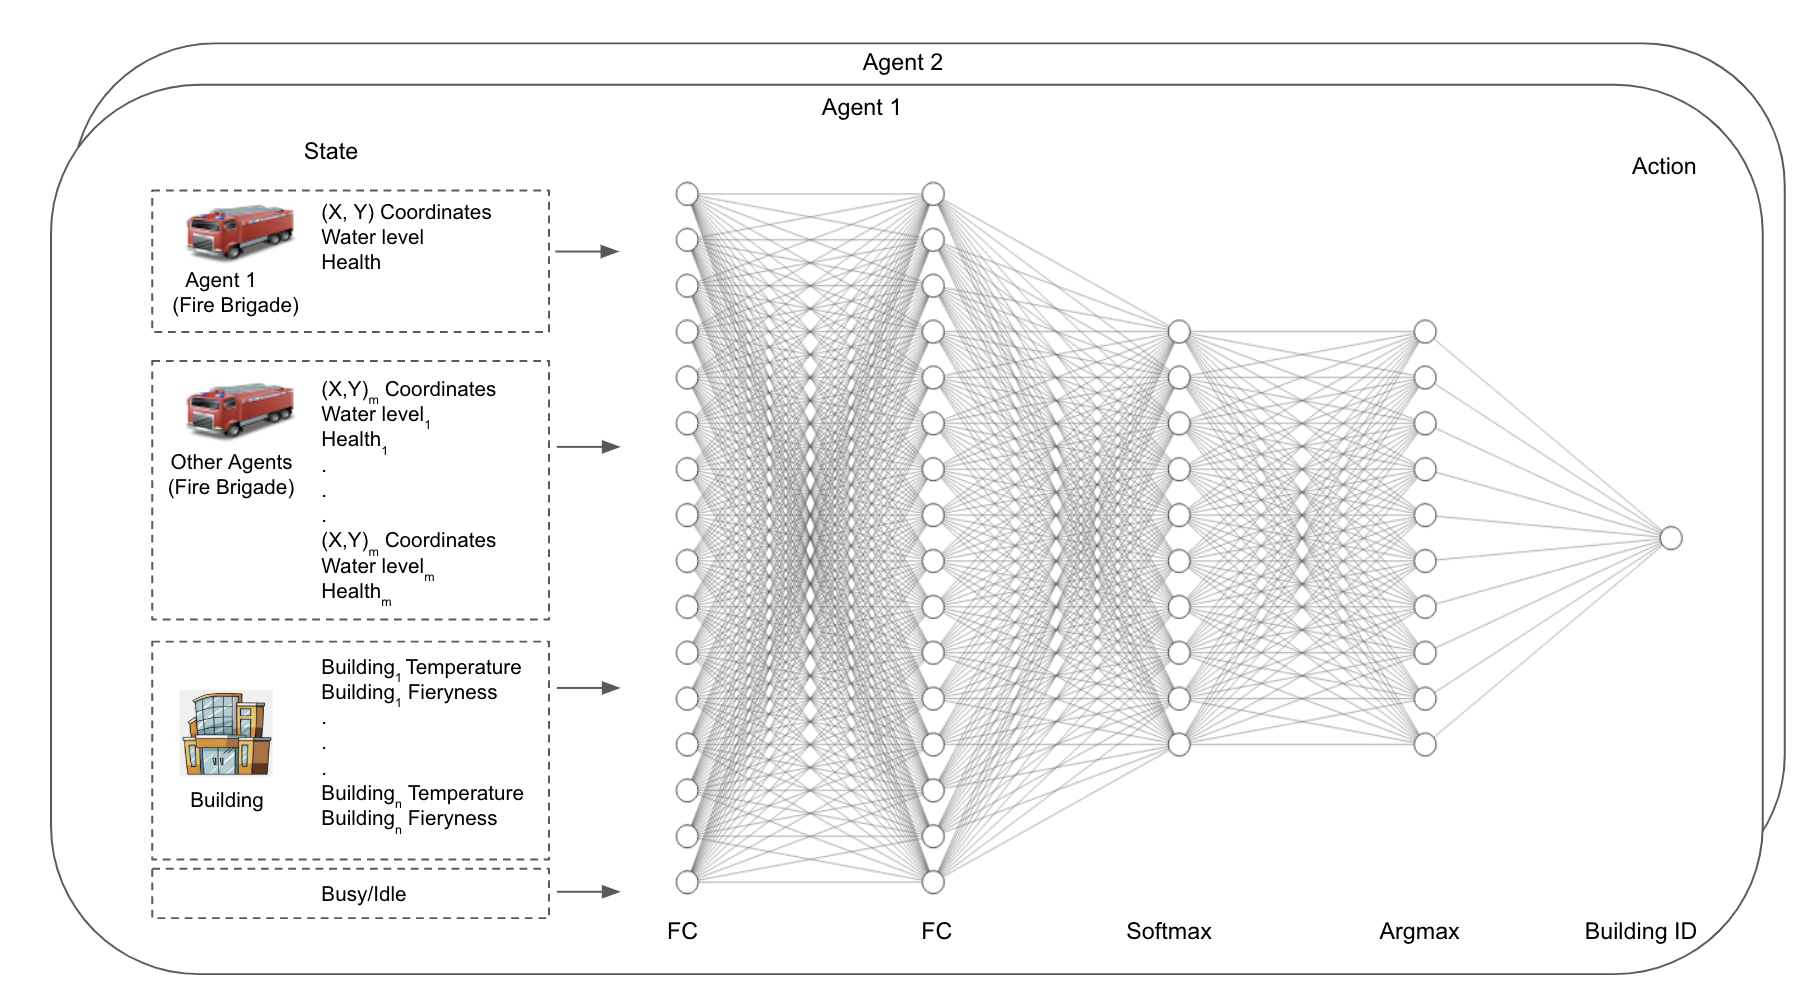
\includegraphics[width=17cm]{27}
    \caption{Schematic Illustration of the Model Architecture}
    \label{fig:27}
\end{figure}

\section{Hyperparameter Search}

For DQN and PPO, different parameter were tweaked like batch size, learning rate, discount factor. For each parameter setting, 5 repetitions were done and the average value of the reward was calculated. Values of the parameter that were tried can be found in Table ~\ref{table:DQNRangesHyperparameter}. 400 episodes were run for "Small" map and 5000 episodes were run for "Big" map. 

\begin{table} [!h]
\begin{center}
 \begin{tabular}{l | l} 
 \hline
 Parameter & Values \\ [0.5ex] 
 \hline\hline
 Discount factor ($\gamma$) & {.99, .993, .997, .999}\\
 n-step & {32, 64, 128, 256}\\
 Entropy Coefficient & 0.01\\
 Learning rate & log-uniform (1e−7 $\rightarrow$ 1e−3) \\
 Value Function Coefficient & 0.5 \\
 Gradient Clipping value & 0.5 \\
 Number of training minibatches & 4 \\
 Clip Range & 0.2\\
 Optimizer & Adam \\ 
 \hline
\end{tabular}
\caption{PPO: Values used during hyper-parameter search and final values used for experiments with scoring}
\label{table:DQNRangesHyperparameter}
\end{center}
\end{table}

\begin{table} [!h]
\begin{center}
 \begin{tabular}{l | l } 
 \hline
 Parameter & Values  \\ [0.5ex] 
 \hline\hline
 Discount factor ($\gamma$) & {.99, .993, .997, .999}\\ 
 Learning rate & log-uniform (1e−7 $\rightarrow$ 1e−3) \\
 Buffer size & {25000, 50000, 100000} \\
 Exploration Fraction & 0.1\\
 Batch size & {32, 64, 128, 256} \\
 Learning starts & {1000, 2000} \\
 Target Network update frequency & 500\\
 Optimizer & Adam \\ 
 \hline
\end{tabular}
\caption{DQN: Values used during hyper-parameter search and final values used for experiments with scoring}
\label{table:PPORangesHyperparameter}
\end{center}
\end{table}

\chapter{RCRS Gym Environment: Setup, Experiments and Results}

In order to device the model presented in Chapter 3 and prove its concepts, an OpenAI gym environment \cite{brockman2016openai} was created that allowed developing agents which are capable of extinguishing fire in the city. 

OpenAI is a framework which defines a standard structure that a DRL agent can be built with, thus making the structure of the agent easy to recognize by any developer and makes the agent compatible with any environment. 

Since OpenAI is built in Python, it can be easily connected with state-of-art DRL framework such as Tensorflow \cite{Abadi} with gym agents and use DRL techniques that use those frameworks provide. There are certain example algorithms available in OpenAI gym which simplifies the testing on a new environment. 

The conceptual model of RCRS gym environment is presented in Figure ~\ref{fig:OpenAIgymRCRS}. Section 4.1 elaborates about the setup that was created to adapt RCRS to allow the training of DRL agents. In Section ~\ref{Experiments}, experiments that were carried out will be detailed and results will be analyzed. 

\begin{figure}[!h]
    \centering
    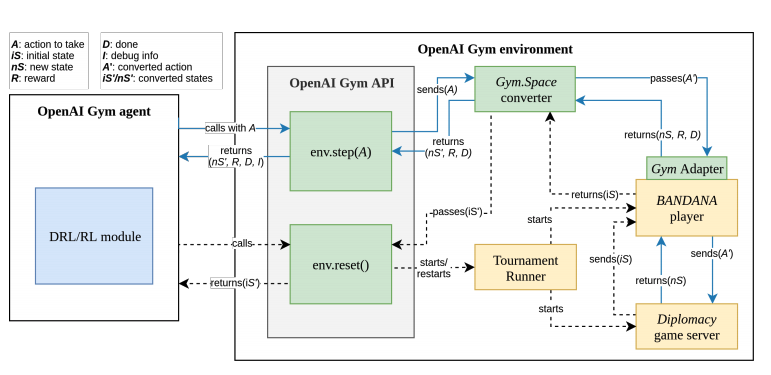
\includegraphics[height=8cm, width=17cm]{OpenAIgymRCRS.png}
    \caption{Conceptual model of the RCRS Gym environment and agent}
    \label{fig:OpenAIgymRCRS}
\end{figure}

\section{Setup} \label{Setup}

This section will deal with the process of building the environment and the logic behind the decisions that are made. 

Section ~\ref{RCRSEnvironment} will describe the goal of the agent, what tasks will it perform after training, introduction to various maps and the complexity of the environment. 

Section ~\ref{OpenAIGym} will elaborate about gym framework and why it was selected.

RCRS is written in Java and OpenAI gym in Python. There has to be a communication channel by which these two languages can communicate in order to send messages. Section ~\ref{CommunicationJavaPython} will discuss about how the communication between Java and Python was established. 

Finally, the overall implementation of RCRS-gym environment will be discussed in Section ~\ref{RCRSGymImplementation}. 


\subsection{RCRS Environment} \label{RCRSEnvironment}

%%%----------------Write Here Something---------------%%%

In order to test the algorithms, two maps were chosen. A "Small" map having fewer number of buildings and fire brigades to fasten the training process and a "Big" map having greater number of buildings and fire brigades. The Map specification can be seen in Table ~\ref{table:RCRSMapSpecs}. The representation of "Small" map can be seen in Figure ~\ref{fig:RepresentationofSimulator} and of "big" map in Figure ~\ref{fig:BigMap}

\begin{table} [!h]
\begin{center}
 \begin{tabular}{l | l | l} 
 \hline
 Map Name & Number of buildings & Number of Agents (Fire Brigades)  \\ [0.5ex] 
 \hline\hline
 Small & 37 & 2\\
 Big & 100 & 4\\
 \hline
\end{tabular}
\caption{RCRS Map Specifications}
\label{table:RCRSMapSpecs}
\end{center}
\end{table}

\begin{figure}[!h]
    \centering
    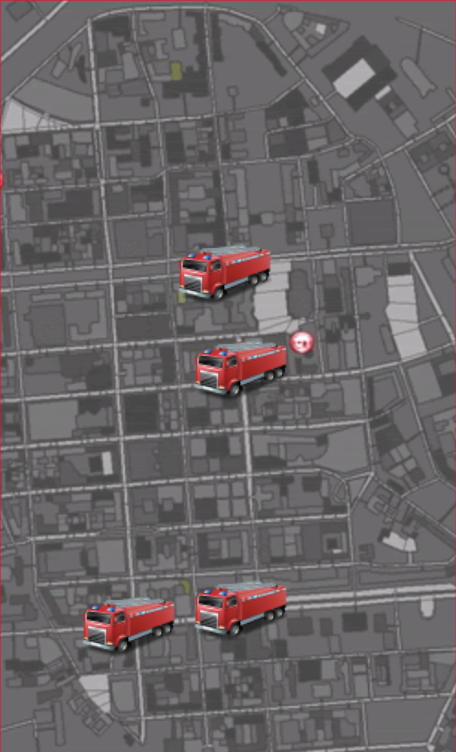
\includegraphics[width=8cm]{BigMap.png}
    \caption{Representation of "Big" Map}
    \label{fig:BigMap}
\end{figure}


\subsection{OpenAI Gym} \label{OpenAIGym}

Having a standard architecture where a reinforcement learning agent can be developed will be really helpful and this is what OpenAI gym provides. This standard architecture helps compare performance of different reinforcement learning algorithms in the same environment \cite{brockman2016openai}. 

OpenAI Gym maintains a repository known as \emph{baselines} \cite{baselines}, which has examples of implementations of state-of-art DRL methods. But baselines have certain drawbacks that \emph{stable baselines} tried to rectify like having a unified structure for all the algorithms, well documented functions and classes and PEP8 compliant. Hence we decided to go with stable baselines \footnote{\url{https://stable-baselines.readthedocs.io/en/master/}}  \cite{stable-baselines}. 

These implementations can be used to validate the environment. The defined gym interface is made of two methods that the agent will use to interact with the environment:

\begin{itemize}
    \item \emph{reset}: This function is used to reset the environment to its initial state and returns the initial observation. It is called whenever a new episode is started. 
    \item \emph{step}: This function receives the action that the agent wishes to use in order to interact with the environment as the argument and returns the observation, reward, done and info. 
    \begin{itemize}
        \item \emph{observation}: Current state information
        \item \emph{reward}: Reward collected after the end of every episode
        \item \emph{done}: returns true if episode is over
        \item\emph{info}: (optional) extra information that needs to be printed
    \end{itemize}
\end{itemize}

In addition to the above attributes, "action space" and "observation space" should be defined in order to abstract the environment to generic code. 

Apart from the above mentioned functions, there are two more important attributes that need to be defined. 

\begin{itemize}
    \item \emph{action space}: The space of possible actions that will be used to generate the actions. Possible values are 
    \begin{itemize}
        \item \emph{Discrete:} A list of possible actions where each timestep only one of the action can be used
        \item \emph{MultiDiscrete:} A list of possible actions where each timestep only one action of each discrete set can be used
        \item \emph{Box:} A N-dimensional box which contains every point in the action space
        \item \emph{MultiBinary:} A list of possible actions, where each timestep any of the actions can be used in any combination
    \end{itemize}
    
    \item \emph{observation space}: The space that defines the dimension of the environment's state. Possible values are the same as listed for action space. 
\end{itemize}

In our case, since the actions are discrete, we selected Discrete action space. States are values that have integers as well as floating numbers between 0 to 15000, we decided to select Box state space that would allow all the values between 0 to 15000 to be possible. 

\subsection{Communication between Java and Python} \label{CommunicationJavaPython}

RCRS is written is Java whereas OpenAI gym is in Python. Since at every timestep, state values have to be sent to the OpenAI gym agent and action values have to be received back, a connection has to be established. This connection between Java classes and Python classes was built using Google's protocol buffers \footnote{\url{https://developers.google.com/protocol-buffers/}}  and gRPC \footnote{\url{https://grpc.io/}}. 

Google's protocol buffers are extensible methods for serializing structures data like XML but is faster, smaller and simpler. They are independent of the programming language they are written in. In our case, protocol buffer's are used to generate methods in python and java so as to use the interpretation of both state space and action space. 

Another important point to note down is that the original structuring of the RCRS code base, already had a server and a client connection which was done using socket programming. The server had all the information of the building state i.e. temperature and fieryness whereas client had the information of the agents i.e. (X,Y) coordinates, health points, water level and if the agent is idle or busy. Client was also the one that would receive the next action to be performed i.e. the next building id where the fire brigades should move to. Since RCRS would have to start first and act as a server to the Python agent, we had to build two servers, one that would send the building information and other that would send the agent information and take actions as well. The Python agent would act as client for these two servers. Listing ~\ref{lst:StateInfo} elaborates the protocol representation of the building information while Listing ~\ref{lst:AgentInfo} elaborates the protocol representation of the agent information. 

\begin{lstlisting} [language=Java, label={lst:StateInfo}, caption=Protocol buffer representation of the Building Information] 
message BuildingInfo {
  int32 fieryness = 1;
  double temperature = 2;
  int32 building_id = 3;
}
\end{lstlisting}

\begin{lstlisting} [language=Java, label={lst:AgentInfo}, caption=Protocol buffer representation of the Agent Information] 
message AgentInfo {
  int32 agent_id = 1;
  double x = 2;
  double y = 3; 
  int32 water = 4;
  int32 hp = 5; 
  int32 idle = 6;
}
\end{lstlisting}

gRPC is an open-source remote procedural call (RPC) framework that can run in any environment. Its ease of implementation and pluggable support for load balancing made it our first choice for serialization. 
RPC server in our case is the gym environment whereas the fire brigade agents acts as RPC clients. Since everything is hidden in the RPC, RCRS (Java classes) will not need to know that it is interacting with the python agent. 

The implementation part is detailed in Listing ~\ref{lst:gRPCBuilding} and Listing ~\ref{lst:gRPCAgent}. 

\begin{lstlisting} [language=Java, label={lst:gRPCBuilding}, caption= gRPC Implementation for Building Info] 
service RCRSGymService {
  rpc getBuildingInfo (Empty) returns (BuildingInfo) {}
}
\end{lstlisting}

\begin{lstlisting} [language=Java, label={lst:gRPCAgent}, caption= gRPC Implementation for Agent Info] 
service RCRSGymService {
  rpc getAgentInfo (ActionInfo) returns (AgentInfo) {}
}
\end{lstlisting}

\subsection{RCRS-Gym Implementation} \label{RCRSGymImplementation}

Lets elaborate on the two methods that were defined in Section ~\ref{OpenAIGym} and show how the agents act in the environment using OpenAI gym. 

First, \emph{reset} function is called. By calling the \emph{reset} function, agent expects the initial state information. To obtain that, RCRS and gRPC server starts. Initial state is always the starting position of the fire brigades which can be pre-decided before running the simulations.

After the simulation starts, gym agent sends a random action to the RCRS server using \emph{step} function which then acts in the environment and sends back the next state information, reward value and if the episode is done or not. Pictorial representation of the working RCRS-gym working is shown in Figure ~\ref{fig:23}. 

An episode is done only after 100 timesteps for "Small" map and after 250 timesteps for "Large" map. The reason for selecting different timesteps for an episode to end was that official RCRS Competition is run for 250 timesteps for "Large" map. But for "Small" map, 250 timesteps was more than enough for all the fire brigades to extinguish the fire in all the buildings. Hence, we decided to reduce that time to 100 timesteps which was sufficient to see if the agents are actually learning or not. 

An example code that will run a random agent in RCRS environment is provided in Listing ~\ref{lst:WorkingofRCRSGym}:

\begin{lstlisting} [language=Python, label={lst:WorkingofRCRSGym}, caption=Example code that will run a random agent in RCRS environment] 
import RCRS_gym
import gym

env = gym.make('RCRS-v2')
env.reset()
done = False
while not done:
    action = env.action_space.sample()
    obs, rew, done, info = env.step(action)

\end{lstlisting}

\begin{figure}[!h]
    \centering
    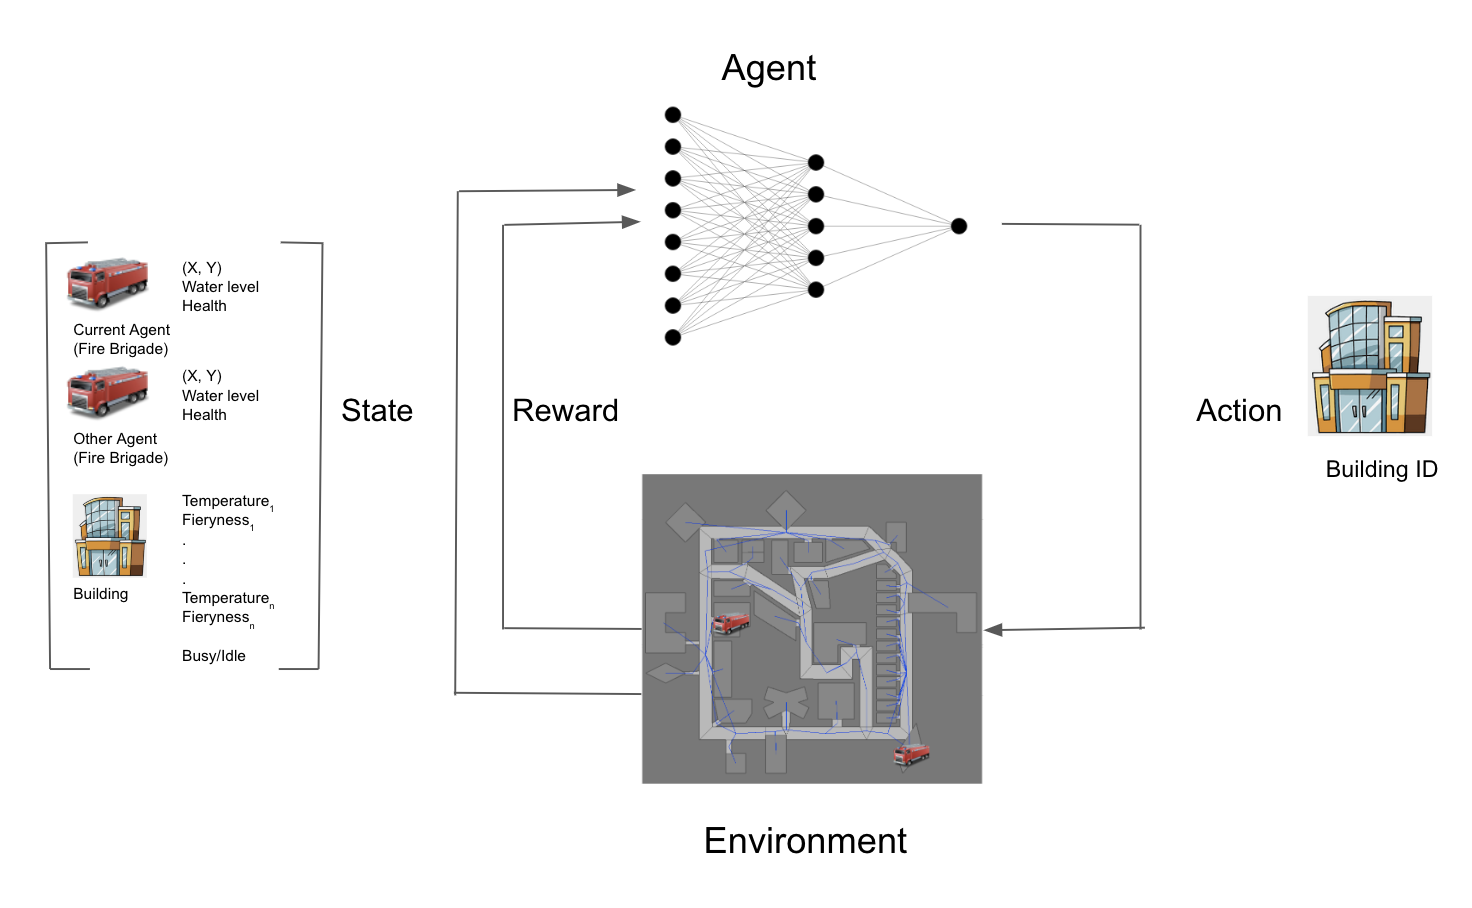
\includegraphics[height=10cm, width=17cm]{23}
    \caption{The neural network takes in state information and the reward collected at every timestep from the environment. State information contains (X,Y) coordinates, water level, health of the all the agents and temperature, fieryness of the buildings present. The neural network processes this information and outputs a building ID where the fire brigade needs to move next}
    \label{fig:23}
\end{figure}

\section{Experiments and Results} \label{Experiments}

To start the testing and see if deep reinforcement learning works on RCRS, we started with experimenting on "Small" map. PPO and DQN algorithm were applied to the simulator and the results were compared with a greedy approach where the agents would always extinguish the building with highest fieryness value. 

\subsection{Small Map Experiments and Results}

Simulations were run for 400 episodes (40,000 timesteps). Out of the several model architectures that were tried, a two hidden layer neural network, each layer having 64 units gave the best results for DQN. For PPO, a neural network having four fully connected layers, where first two layers had 128 units and last two layers had 64 units gave the best result along with the use of LSTM. Best hyperparameters are listed in Table ~\ref{table:BestDQNHyperparameter}
and Table ~\ref{table:BestPPOHyperparameter}. 

\begin{table} [!h]
\begin{center}
 \begin{tabular}{l | l} 
 \hline
 Parameter & Best - Small Map  \\ [0.5ex] 
 \hline\hline
 Discount factor ($\gamma$) & 0.99  \\
 n-step & 32\\
 Entropy Coefficient & 0.01\\
 Learning rate & 5e-4\\
 Value Function Coefficient & 0.5\\
 Gradient Clipping value &  0.5\\
 Number of training minibatches & 4\\
 Clip Range & 0.2\\
 Optimizer & Adam  \\ 
 \hline
\end{tabular}
\caption{PPO: Best hyperparameters}
\label{table:BestDQNHyperparameter}
\end{center}
\end{table}

\begin{table} [!h]
\begin{center}
 \begin{tabular}{l | l} 
 \hline
 Parameter & Best - Small Map  \\ [0.5ex] 
 \hline\hline
 Discount factor ($\gamma$) & 0.99 \\ 
 Learning rate & 5e-4\\
 Buffer size & 50000 \\
 Exploration Fraction & 0.1\\
 Batch size  & 64\\
 Learning starts & 1000\\
 Target Network update frequency & 500\\
 Optimizer & Adam \\ 
 \hline
\end{tabular}
\caption{DQN: Best hyperparameters}
\label{table:BestPPOHyperparameter}
\end{center}
\end{table}

Mean and standard deviation of the reward is calculated after every 5 episodes. Since greedy algorithm wasn't learning, it had a constant reward value of 6.33. DQN achieved a highest cumulative reward of 5.89 and PPO achieved a highest cumulative reward of 5.88. Figure ~\ref{fig:SmallMapResults} shows that both the algorithms were able to learn in the environment improving their cumulative rewards over time. However, DQN attained highest cumulative reward in less number of episodes than PPO showing that it is a more effective algorithm for "Small" map setting.  

Figure ~\ref{fig:PPOLearningSmallMap} and Figure ~\ref{fig:DQNLearningSmallMap} show how the agents gets better at extinguishing fire over the episodes. After 5 episodes, both the algorithms were performing badly with most of the buildings critically or totally burnt. After 150 episodes, agents started learning and higher number of buildings were extinguished. After 250 episodes, DQN was able to successfully figure out the buildings that caused the fire to spread throughout the map and was able to extinguish fire in those buildings. PPO was performing better than how it was performing after 150 episodes, but still not as good as DQN. After 300 episodes, PPO was also able to successfully extinguish the critical buildings. For better visualization on how the agents performed over episodes, refer to the \href{https://github.com/animeshgoyal9/RoboCup_Rescue_Simulator_Gym_Integration} {GitHub page}. 

\begin{figure}[!h]
    \centering
    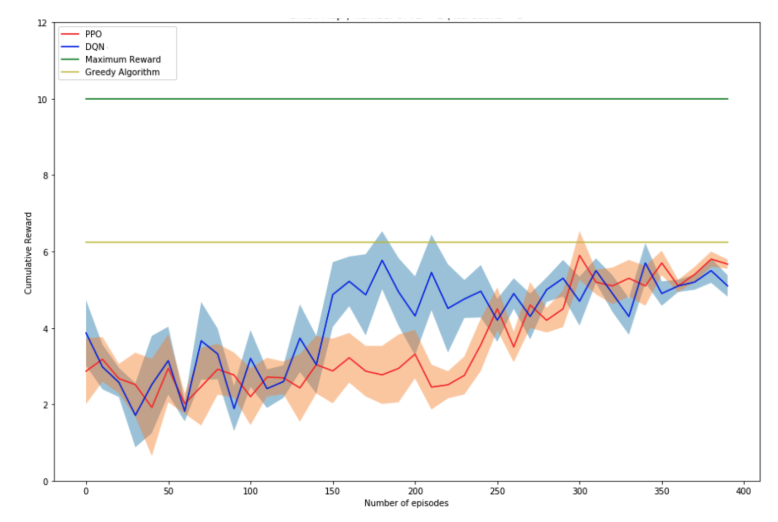
\includegraphics[width=12cm]{29.png}
    \caption{Rewards per episode for PPO, DQN and Greedy algorithm in "Small" Map setting. Dark line represents the mean value for rewards while shaded region is the standard deviation}
    \label{fig:SmallMapResults}
\end{figure}

\begin{figure}[!h]
    \centering
    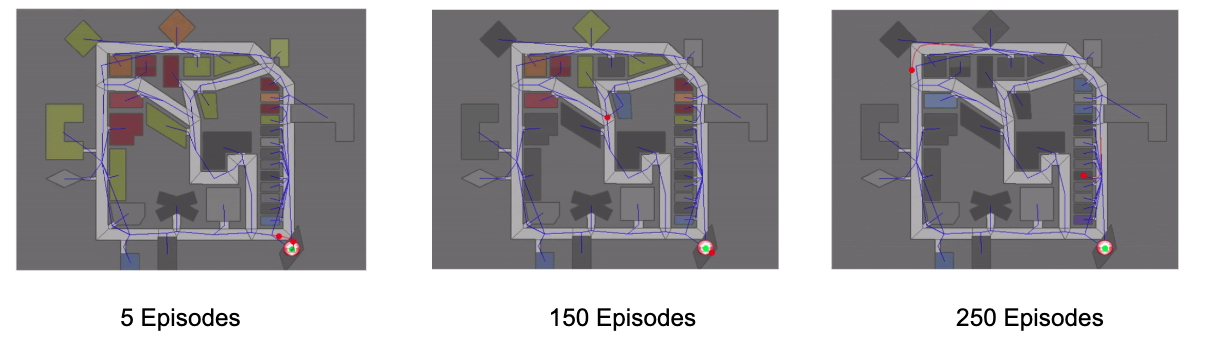
\includegraphics[width=17cm]{PPO.png}
    \caption{PPO: Fire Brigades learning to extinguish fire over 250 episodes. After 5 episodes, there was hardly any learning with most of the buildings either critically or totally burnt. After 250 episodes, agents learnt the critical buildings that need to be extinguished}
    \label{fig:PPOLearningSmallMap}
\end{figure}

\begin{figure}[!h]
    \centering
    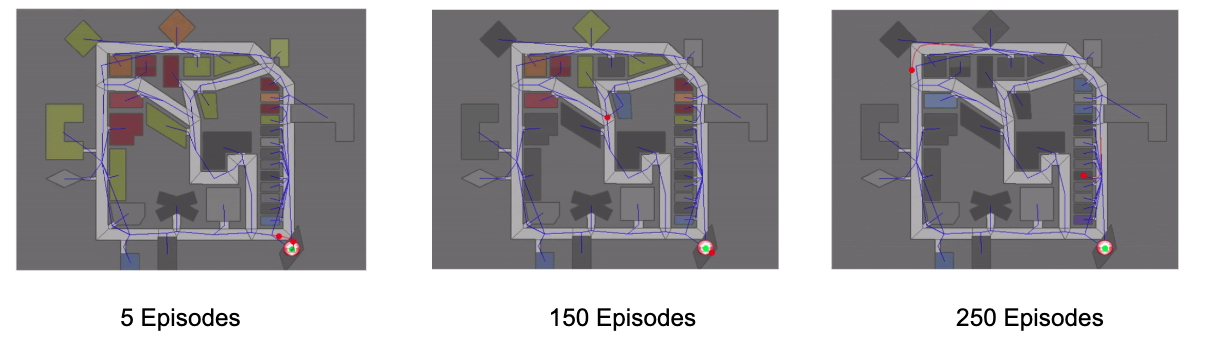
\includegraphics[width=17cm]{DQN.png}
    \caption{DQN: Fire Brigades learning to extinguish fire over 250 episodes. After 5 episodes, there was hardly any learning with most of the buildings either critically or totally burnt. After 250 episodes, agents learnt the critical buildings that need to be extinguished}
    \label{fig:DQNLearningSmallMap}
\end{figure}

\subsection{Big Map Experiments and Results}
---------------------------------Still in progress---------------------------------

% \begin{figure}[!h]
%     \centering
%     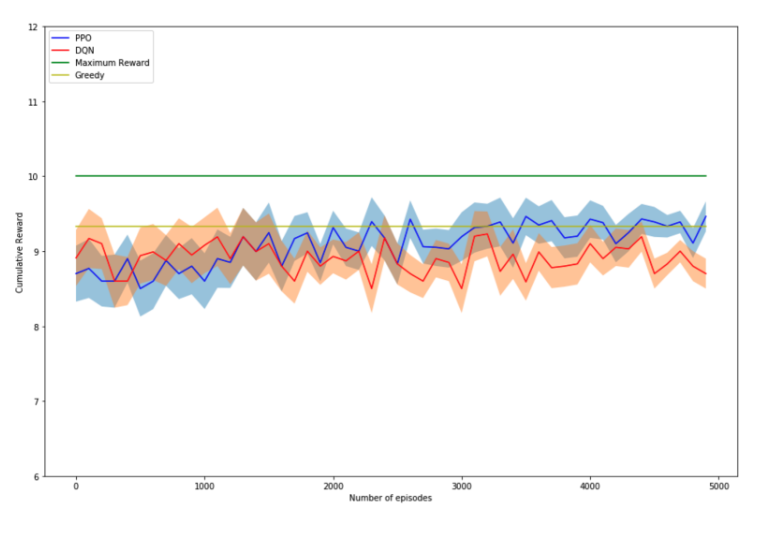
\includegraphics[width=12cm]{30.png}
%     \caption{Comparison of Results for Big Map}
%     \label{fig:DQNSmallMapLearningMaps}
% \end{figure}

\chapter{Conclusion and Future Work}

In this report, we have presented how deep reinforcement learning can be applied to a multiagent scenario, specifically to RoboCup Rescue Simulator.We have built a RCRS-gym interface that will allow different RL algorithms to be applied to the simulator. The interface created provides an easy setup for developers to research RCRS using Python framework. The gRPC communication between Java and Python is also a feature that proved important to send actions and receive state information. 

We evaluated two state-of-the-art DRL algorithms, Proximal Policy Optimization (PPO) and Deep Q-Networks (DQN). Both the algorithms were trained on two map setting: "Small" map and "Big" map. 

PPO and DQN were both able to demonstrate learning on the "Small" map with average cumulative reward increasing over episodes. DQN converged quickly than PPO showing that it performed better as compared to PPO. However, these algorithms were slightly subpar when compared to Greedy algorithm where the agents would always extinguish the building with highest fieryness value. 

This study demonstrated that successfully trained agents can indeed learn a strategy to extinguish the buildings on fire proving that RCRS is a suitable environment to apply Deep Reinforcement learning techniques. However, there are various avenues that can be studied as future research. Applying similar techniques for a bigger map setting can be the first line of direction of study for researchers. Is there a map setting where PPO and DQN performs better than greedy algorithm, are there situations where PPO learns quicker than DQN, can this be generalized by looking at the number of buildings in the map, are some of the questions that are still unanswered. 

Another avenue to research for is how can we include other agents like police officers and ambulance teams to train them and accomplish their individual tasks successfully. Our current work assumes full observability to all the agents, future work can also focus on training the agents with partial observability. 


%\addcontentsline {toc}{chapter}{Bibliography} 
                                     %% Force Bibliography to appear in contents

\bibliographystyle{plain}
\bibliography{bibliography.bib}      

\end{document}                       %% Done.
